\RequirePackage{plautopatch}
\documentclass[uplatex,dvipdfmx,a4paper]{jsarticle}
\usepackage{ics-thesis}

% ===== Other packages =========================================================
\usepackage{otf}
\usepackage[hiresbb]{graphicx}
\usepackage{url}
\usepackage{multirow}
\usepackage{amssymb}
\usepackage{array}
\usepackage{arydshln}
\usepackage{multirow}
\usepackage{listings}
\usepackage[svgnames]{xcolor}
\usepackage{lscape}
\usepackage[caption=false,font=footnotesize]{subfig}
\usepackage{dblfloatfix}
\usepackage{ascmac}
\usepackage{xspace}  % for cite

% ==============================================================================

% ===== Package settings =========================================================
\definecolor{diffstart}{named}{Grey}
\definecolor{diffincl}{named}{Green}
\definecolor{diffrem}{named}{Red}

\lstdefinelanguage{diff}{
  basicstyle=\ttfamily\footnotesize\color{darkgray},
  frame=single,
  linewidth=1.00\textwidth,
  morecomment=[f][\color{diffstart}]{@@},
  morecomment=[f][\color{diffincl}]{+},
  morecomment=[f][\color{diffrem}]{-},
}
\lstset{
  language=diff,
  basicstyle=\ttfamily\footnotesize\color{darkgray},
  frame=single,
  linewidth=1.00\textwidth,
  breaklines=true,
  keywordstyle=\textbf,
  commentstyle=\color{green},
  keywordstyle=\color{blue},
  stringstyle=\color{red},
  tabsize=2,
  lineskip=-0.3zw
}

\hdashlinewidth=0.5pt
\hdashlinegap=1.0pt
% ==============================================================================


% リファレンス参照コマンド
\newcommand{\figref}[1]{図~\ref{#1}}
\newcommand{\tabref}[1]{表~\ref{#1}}
\newcommand{\chapref}[1]{\ref{#1}~章}
\newcommand{\secref}[1]{\ref{#1}~節}
\newcommand{\subsecref}[1]{\ref{#1}~項}

% ハイライトコマンド
\newcommand{\unmodified}[1]{{\textcolor{red}{#1}}}
\newcommand{\modified}[1]{{\textcolor{blue}{#1}}}
\newcommand{\needChange}[1]{{\textcolor{magenta}{#1}}}
\newcommand{\comment}[1]{{\textcolor{darkgray}{#1}}}
\newcommand{\TODO}[1]{{\textcolor{green}{#1}}}
% red,green,blue,cyan,magenta,yellow,black,gray,white,darkgray,lightgray,brown,lime,olive,orange,pink,purple,teal,violet

% footnote用のカウンタ
\newcounter{fcounter}
\setcounter{fcounter}{1}
\newcommand{\fcount}{\the\value{fcounter}\stepcounter{fcounter}}
\newcommand{\fcountin}{\the\value{fcounter}}

\let\oldcite\cite
\renewcommand{\cite}[1]{\xspace\oldcite{#1}}

% ===== Title page configuration ===============================================
\pagestyle{bachelorthesis}
\title{遺伝的アルゴリズムを用いた自動プログラム修正における\\個体生成時間の計測とその分析}
\author{皆森 祐希}
\supervisor{楠本 真二 教授}
\deadline{令和5年2月7日}
% ==============================================================================

\begin{document}

\titlepage

\pagestyle{empty}
\abstract {
  ソフトウェア開発において,デバッグは開発工数の半分を占める作業といわれている.自動プログラム修正は,バグを含むプログラムに変更を加えることで用意したテストを通過するプログラムを出力する手法であり,デバッグの工数を削減することが期待されることから研究が盛んに行われている.
  自動プログラム修正の手法として,遺伝的アルゴリズムに基づいて修正を行うものがある.
  ここで,自動プログラム修正における遺伝的アルゴリズムは,目的のプログラムが得られるまでプログラム文の挿入,削除,置換及び交叉を行う手法である.
  現状の自動プログラム修正における課題の1つとして,1つのバグに対する修正に長い時間がかかる点があげられる.しかし,現状の自動プログラム修正ツールにはバグ修正時間のうち個体生成に対する計測機能が存在しない.
%Macawは,遺伝的アルゴリズムを採用したAPRツールのひとつであるkGenProgの進化過程をツリー状に可視化するツールであり,遺伝アルゴリズムにおける膨大な変異プログラムの解析を容易にすることが期待される.しかし,kGenProg及びMacawには個体の生成時間を計測および表示する機能が実装されておらず,解となる経路が最適に生成されているかどうかを確かめることが困難である.
  そこで,本研究では遺伝的アルゴリズムを採用した自動プログラム修正ツールのひとつであるkGenProgに各個体の生成にかかった時間を計測する処理を追加した.さらに得られた個体情報をビルドの成否および解であるかどうかに分類した.その後,全体の生成時間のうち解となるプログラムの生成経路にかかった時間およびビルドに失敗した個体に費やした時間を定量的に計算することで,自動プログラム修正の時間的コストを調査した.
}

\keyword {
  自動プログラム修正, 時間計測,可視化,  JSON
}

% 目次
\clearpage
\pagestyle{plain}
\pagenumbering{roman}
\tableofcontents

% 図目次
\clearpage
\listoffigures

% 表目次
\clearpage
\listoftables

% 本文
\clearpage
\pagenumbering{arabic}

\newcommand{\kgp}{kGenProg}
\newcommand{\mcw}{Macaw}
%%%%%%%%%%%%%%%%%%%%%%%%%%%%%%%%%%%%%%%%%%%%%%%%%%%%%%%%%%%%%%%%%%%%%%%%%%%%%%%%%%%%%%%%%%%%%%%%%%%
\clearpage
\section{はじめに}\label{sec:intro}
ソフトウェア開発におけるデバッグ作業は費用および時間的な点で多くのコストを必要とする.ある研究によると,ソフトウェア開発にかかるコストのうち,50\%以上をデバッグが占めるという結果が出ている\cite{5386906, Britton_reversibledebugging}.
自動プログラム修正(APR)は,人の手を介さずにソースコード中に含まれるバグを自動的に取り除く技術であり,盛んに研究が進められている\cite{gazzola2018automatic, goues2019automated}.
%APRは大きく探索ベースの手法と意味論ベースの2つの手法に分類することができるが,本研究では,探索ベース
APRの実用化に向けて,ここ10年で数多くの研究がなされており,特にコストを削減する取り組みも行われている\cite{id692,qi2013efficient}.しかし,先行研究においては個体の生成時間の削減に関する研究は多くない.そこで,本稿では,既存のAPRツールを拡張して個体の生成時間を計測し,筆者が考案した指標を実際のバグに対して計算することで時間的コストを調査する.\\
以降,\ref{sec:prep}章ではAPRの課題本研究を行う契機となった研究の説明および研究のための予備知識について説明する.
\ref{sec:sgst}章では本研究における提案手法について論じる.
\ref{sec:prop}章では今回提案した評価指標とその具体例について論述する.
\ref{sec:exp}章では実験の概要と結果を提示する.
\ref{sec:cons}章では実験から得られた結果による考察について述べる.
\ref{sec:threat}章では本研究の妥当性への脅威について論じる.
\ref{sec:ftrclg}章では今後の課題について説明し,
最後に\ref{sec:concl}章で総括を述べる.
%%%%%%%%%%%%%%%%%%%%%%%%%%%%%%%%%%%%%%%%%%%%%%%%%%%%%%%%%%%%%%%%%%%%%%%%%%%%%%%%%%%%%%%%%%%%%%%%%%%

\clearpage
\section{準備}\label{sec:prep}
%本章では,遺伝的アルゴリズム(GA)に基づく自動プログラム修正(APR) の生成過程について述べる.
\subsection{自動プログラム修正(APR)}\label{sec:apr}
APRは,テストケースとバグを含むプログラムを入力として,計算機が自動的にプログラムのバグ修正を行う技術である.この時,入力したプログラムを修正したプログラムを出力とする.APRは大きく探索ベース\footnote{Heuristics-based}と意味論ベース\footnote{Semantics-based}\cite{le2018overfitting}の2つの手法に分類することができるが,本研究では,探索ベースAPR分野のブレイクスルーとなったGenProg\cite{le2011genprog}の採用する生成と検証\cite{martinez2019astor}に基づく手法に重点を置く.\\
この手法では,図\ref{fig:apr}のように,対象となるプログラムにおけるバグの位置を特定する手法である欠陥限局を行い,限局した箇所に変更を加えた後ビルドとテストを実行して修正尺度の評価を行う.
\begin{figure}[t]
  \centering
  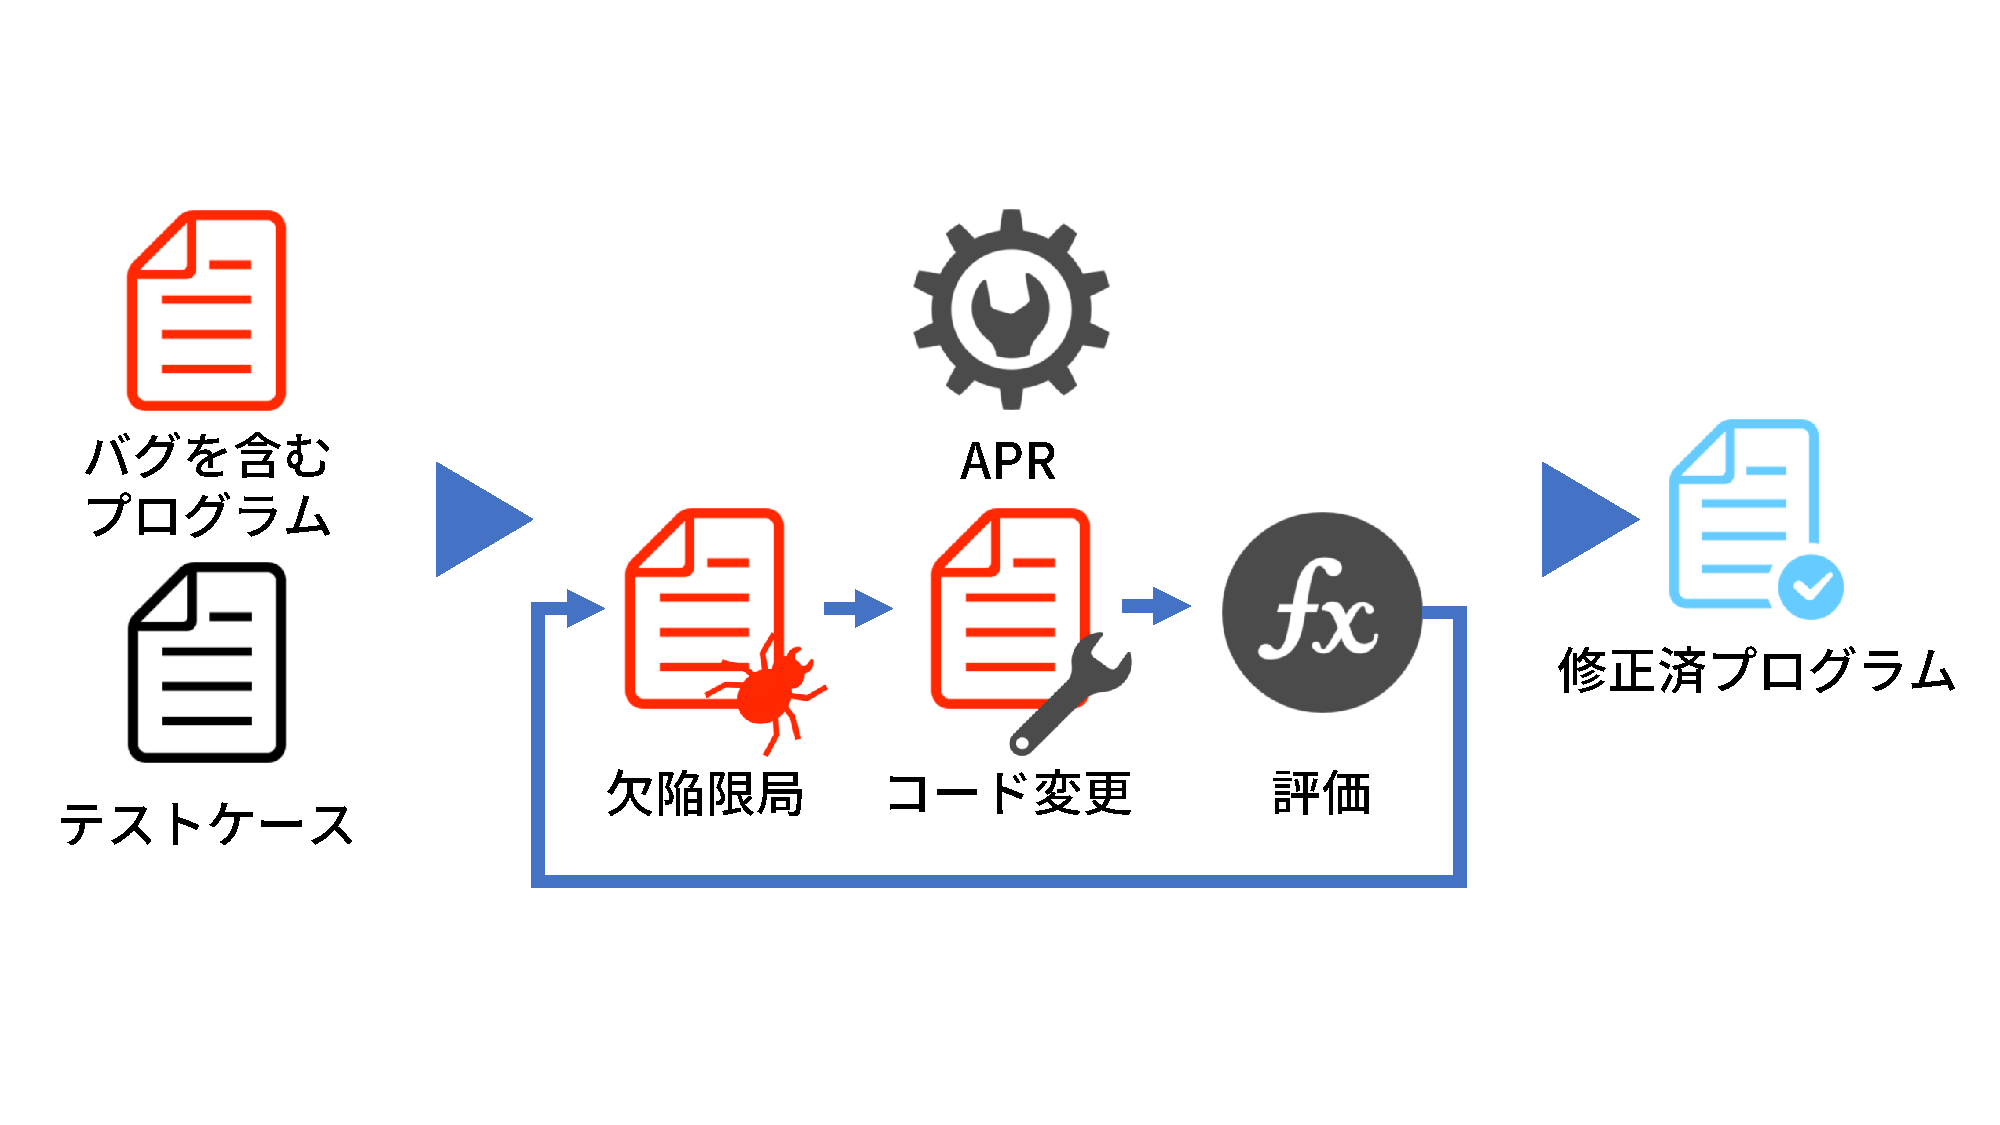
\includegraphics[width=\linewidth]{fig/apr.pdf}
  \caption{自動プログラム修正 : APR}
  \label{fig:apr}
\end{figure}
\subsection{遺伝的アルゴリズム}\label{sec:ga}
遺伝的アルゴリズム(GA)は各世代で個体を選択し,それらに変異,交叉などの操作を加えることでより強い個体を生成する生物の進化に基づくアルゴリズムである.これらの個体から以下の遺伝子操作を行うことで,次の世代の個体の集合を生成する.
\begin{description}
\item{選択} …個体のうちから何らかの関数による適応度(APRではテストスイートの通過率)に応じて選択
\item{変異} …個体の遺伝子を変異させる(APRではコードの一部を変更)
\item{交叉} …複数の遺伝子の一部分を交配させて新しい遺伝子を生成
\end{description}
これらの遺伝子操作のうち,変異においてAPRでは以下の操作を対象のコードに対して行う.\\
\begin{description}
\item{挿入} …選択したコード近辺への別コードの追加
\item{置換} …選択したコードの別コードへの書き換え
\item{交叉} …選択したコードの削除
\end{description}
遺伝的アルゴリズムの具体的な説明として,図\ref{fig:ga}のような遺伝について考える.なお,図中の数字はテストスイートの通過率(以下,単に通過率と表す)を表し,もっとも左の個体群を第1世代として,右に行くほど世代が進んでいるものとする.\\
第1世代においては,通過率0.5の個体を選択したもの,通過率0.3の個体に変異を起こしたもの,そして通過率0.4と0.3の個体を交叉したものの3つの個体を第2世代の個体として生成している.同様に,第3世代の個体は,第2世代の個体のうち,通過率0.7の個体の選択およびこの個体と通過率0.5,通過率0.6の個体との交叉による個体となっている.ここで,第3世代の個体に通過率1.0の個体が存在するのでここでアルゴリズムを終了する.
\begin{figure}[t]
  \centering
  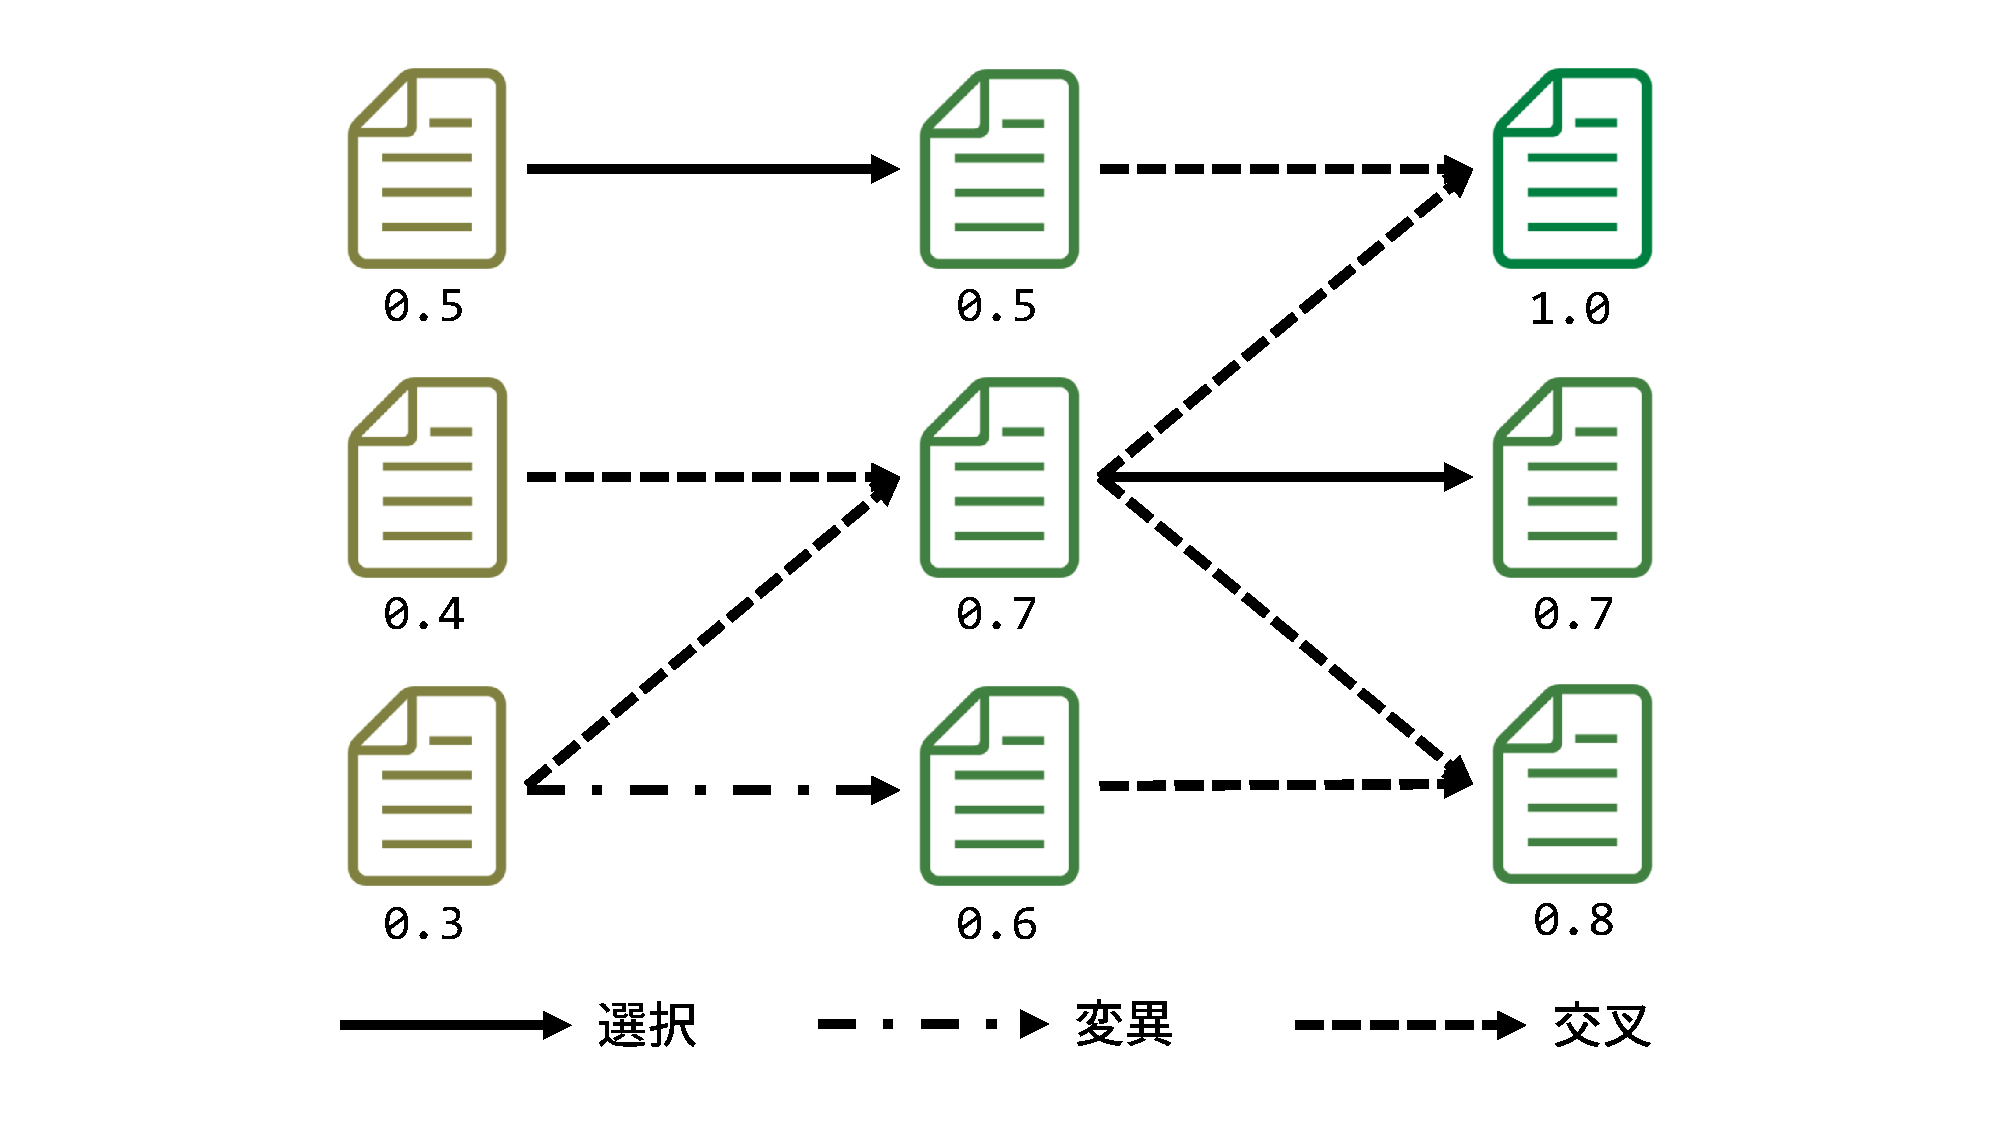
\includegraphics[width=\linewidth]{fig/ga.pdf}
  \caption{遺伝的アルゴリズムの例}
  \label{fig:ga}
\end{figure}
\subsection{既存のAPRツールの課題} \label{sec:prev_challenge}
既存のAPRツールは多くの課題が解決されておらず\cite{le2013current},実用には程遠い段階である.具体的には,修正後のプログラムの可読性が低い\cite{smith2015cure},単一のバグの修正は行えてもバグが複数になると修正が困難になる\cite{saha2019harnessing}などがあげられる.\\
その中で今回主に取り上げる課題として,1回の修正実行にビルドやテスト実行といった多くの時間的コストがかかる点\cite{chen2017contract}があげられる.この課題の動機として,筆者が実際にAPRツールを実行したときに比較的単純なプログラムを対象とした修正において手動でバグを修正したときよりも時間的コストがかかったことがあげられる.
また,ビルドとテストにかかる時間を削減する研究が過去に行われているものの\cite{id692}
%テストの実行時間を計測する機能は実装されているものの
,個体の生成にかかった時間を計測することに関する研究はまだ発展途上である.
\subsection{時間的コスト調査の先行研究}
Ghanbari\cite{ghanbari2019practical}らは従来のソースコード解析に基づいたAPRを実行した後に,バイトコードにAPRを施すPraPRを提案し,既存のAPRの性能を飛躍的に向上させた.この研究において,GhanbariらはPraPRをDefects4JのChartおよびClosureリポジトリに含まれるバグに対して修正を行うとともに時間的コストを計算した.結果として,Closureリポジトリのバグでは有効なパッチ(修正されたプログラム)の数がChartリポジトリのバグに比べて10倍生成されたものの,時間的コストは20倍かかった.
また,古藤\cite{id692}らは欠陥限局を用いて変更コード片を動的に切り替える手法を提案しビルドに費やす時間を従来手法に比べて89\%から46\%に削減することができ,結果としてAPR全体の修正時間の削減につながった.
これらの研究ではプログラム修正全体やビルド時間の観点から時間的コストの調査を行っていたが,自動プログラム修正の時間的コストについて別の観点から詳らかに調べてみようと思い,本研究をするに至った.
%%%%%%%%%%%%%%%%%%%%%%%%%%%%%%%%%%%%%%%%%%%%%%%%%%%%%%%%%%%%%%%%%%%%%%%%%%%%%%%%%%%%%%%%%%%%%%%%%%%
\clearpage
\section{提案手法} \label{sec:sgst}
前の章でも述べた通り,APRツールにおける個体の生成にかかった時間に重点を置いた研究はまだ少ない.
そこで,本研究ではの遺伝的アルゴリズムを採用したGenProg\cite{le2011genprog}系のAPRツールの個体処理部分に時間計測用のコードをはさんで,記録された生成時間を独自の指標で評価する手法を提案する.
%%%%%%%%%%%%%%%%%%%%%%%%%%%%%%%%%%%%%%%%%%%%%%%%%%%%%%%%%%%%%%%%%%%%%%%%%%%%%%%%%%%%%%%%%%%%%%%%%%%
\clearpage
\section{評価指標とその実装} \label{sec:prop}
\subsection{評価指標}\label{sec:index}
\subsubsection{STR}\label{sec:STR}
APRを実行するにあたり,修正に成功したバグに対して,その解となる個体に関係する経路の全体の生成時間に占める割合を求める指標として,{\bf STR}(Solution Time Ratio, 解時間比率)を次の式で定義する.
\begin{equation}
\label{eq:STR} {\rm STR} =  \frac{解となる個体の経路の総生成時間}{すべての個体の総生成時間}
\end{equation}
ここで,解となる個体の経路の集合は
\begin{enumerate}
\item まず解である個体を選択し,集合に入れる \label{sol:step1}
\item 集合内の全個体に対してその親を求め,それらを集合に入れる \label{sol:step2}
\item 集合に変化がなくなるまで\ref{sol:step2}を繰り返す \label{sol:step3}
\end{enumerate}
のように求められる.STRを計算する目的として,プログラム修正において成功に必要な個体の生成が時間的にどの程度の割合を占めているのかを定量的に求めることがあげられる.そのため,STRの値は大きい方が好ましい.
\subsubsection{FTR}\label{sec:FTR}
一方で,すべてのバグに対してビルドに失敗する個体がすべての個体の生成時間に占める割合を求める指標として,{\bf FTR}(Failure Time Ratio, 失敗時間比率)を次の式で定義する.
\begin{equation}
\label{eq:FTR} {\rm FTR} =  \frac{ビルドに失敗した個体にかかった総生成時間}{すべての個体の総生成時間}
\end{equation}
FTRを計算する目的として,プロジェクト内のバグを含むプログラムの修正にかかる時間のうちがどの程度の割合を占めるかを定量的に測定し,その傾向を知ることがあげられる.そのため,一般的にFTRの値は小さい方が望ましいとされる.
\subsection{STR・FTRの具体的な計算例}
先ほど定義した値を求めるための具体的な例として,図\ref{fig:example}の生成木をもつ修正結果について考える.この生成木は,kGenProgの実行結果を記したJSONファイルをツリー状に表示する\mcw \cite{tomida2019visualizing}を参考に描画した\footnote{ビルドに失敗した個体集合を表すX印における数字の意味合いとして,この例では生成時間の和を表すが\mcw においては個体の数を指すなどの細かい違いがある点に注意}.
\begin{figure}[t]
  \centering
  \includegraphics[width=\linewidth]{fig/astSample.pdf}
  \caption{生成結果の例}
  \label{fig:example}
\end{figure}
ここで,縦方向は世代を表しており,下に進むにつれてより新しい世代を表す.また,横の列は一つの世代におけるすべての個体を表す.円及びX印はそれぞれビルドに成功した1つの個体,その世代でビルドに失敗したすべての個体を表す.円の色は個体のFitness(全体のテストケースに占める期待通りのテスト結果が得られた割合)を表し,緑に近いほど高いFitnessを右下の数字はその個体あるいは個体の集合の生成時間を表す.なおこの例におけるプログラムの総生成時間は800である.
この時,STRは図\ref{fig:example_STR}で表される部分の時間$(10 + 15 + 5 + 100 + 200) \div 800 = 0.4125$となり,FTRはX印で示されたすべての時間を足した値を総生成時間で割ったもの,すなわち$(150 + 250) \div 800 = 0.5$と求められる.
\begin{figure}[t]
  \centering
  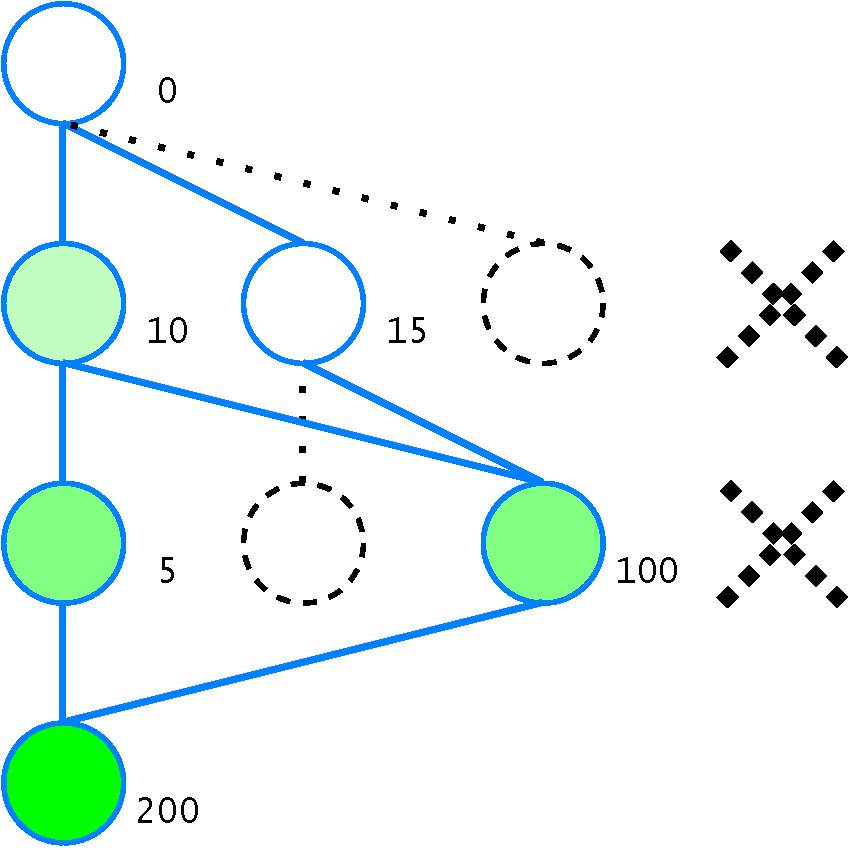
\includegraphics[width=\linewidth]{fig/astSample_STR.pdf}
  \caption{生成結果の例}
  \label{fig:example_STR}
\end{figure}
\subsection{APRツールへの時間計測機能実装} \label{sec:impl}
提案手法では,既存のAPRツールであるkGenProg\cite{higo2018kgenprog}を拡張して実装する.
ソースコード内部のふるまいは変えずに,\texttt{Mutation}クラスと\texttt{RandomCrossover}クラスに時間計測を行うコードを挿入した.具体的には,\texttt{org.apache.commons.lang3.time.StopWatch}クラスをインポートし,各個体を生成するループの最初に\texttt{StopWatch.createStarted()}メソッドを呼び出すことによって時間計測を開始,処理を終えた後に\texttt{getTime()}メソッドを呼び出すことで生成時間を取得し,それを個体情報に格納する.この際,kGenProgに付属しているJSONファイルの出力オプションをオンにすることで対象のバグにおける個体の解析を可能にする.\\
次に,JSONファイルをPythonで記述したプログラムを用いて処理し,各個体のID(通し番号)・生成時間・Fitness(ただしここではIDに対応する個体がビルドに失敗した場合-1を格納する)の情報を取得した後,その情報をもとにSTRとFTRを計算する.\\
具体的には,出力となるJSONファイルを読み込み,バグの修正過程から生成された個体の時間を1つずつ取得する.この時,Fitnessの値で追加の処理を行う.例えばFitnessが-1であればビルドに失敗した個体であるので失敗時間(FTRを計算する際の分子)に加算する.また,Fitnessが1であれば,テストケースを満たす解となる個体であるので\ref{sec:STR}で挙げた手順で解となる個体の親を求める.プログラム中では再帰的なアルゴリズムを用いている.\\
%%%%%%%%%%%%%%%%%%%%%%%%%%%%%%%%%%%%%%%%%%%%%%%%%%%%%%%%%%%%%%%%%%%%%%%%%%%%%%%%%%%%%%%%%%%%%%%%%%%
\clearpage
\section{実験} \label{sec:exp}
\subsection{概要}
本章では,GAを採用したAPRツールであるkGenProg\cite{higo2018kgenprog}を用いて,Defects4J\cite{just2014defects4j}のLangバグのLang1~Lang44を対象に自動プログラム修正を行った.そのうち,ビルドに成功し,かつ解を得ることができたLang6, 
%Lang10,
 Lang22, Lang25およびLang39の
%5
4つのバグを対象として先ほど定義したSTRとFTRを計算し,その値を確認する.なお,生成時間には不確定性があるため各バグごとにAPRを複数回実行している.
表\ref{tab:apr_setting}にAPRツール実行時の設定を,表\ref{tab:project_setting}に実行回数や解に至るまでの総個体数など,各バグに対する実験の条件を示す.
\begin{table}[b]
  \centering
  \caption{APRツールの設定}
  \label{tab:apr_setting}
  \begin{tabular}{ll} \hline\hline
    項目         & 値                           \\\hline
    実験題材     & Defects4J Lang6, Lang22, Lang25, Lang39 \\
    題材数       & 4                           \\
    1世代ごとの変異個体数 & 70 \\
    1世代ごとの交叉個体数 & 30 \\
    乱数シード   & 2       \\
    実験環境     & Corei5-1240P 16GB mem  \\\hline\hline
  \end{tabular}
\end{table}
\begin{table}[b]
  \centering
  \caption{各バグの詳細}
  \label{tab:project_setting}
  \begin{tabular}{lllll} \hline\hline
    バグ名 & Lang6 & Lang22 & Lang25 & Lang39  \\\hline
    到達世代数 & 1 & 7 & 1 & 4 \\
    個体数 & 8 & 624 & 38 & 300 \\
    ビルド失敗個体数 & 7 & 511 & 36 & 274 \\
    サンプル数 & 100 & 15 & 70 & 40 \\\hline\hline
  \end{tabular}
\end{table}
ここで,サンプル数がバグによって異なるのは,1回のプログラム修正にかかる総時間が異なるためである.
\subsection{実験結果}
\subsubsection{Lang6}
図\ref{fig:Lang6_boxplot}にLang6におけるSTRとFTRの箱ひげ図を,表\ref{tab:Lang6}にSTRとFTRの平均(以降AVG),最小値(以降MIN),第1四分位数(以降1Q),中央値(以降MED),第3四分位数(以降3Q),最大値(以降MAX)の各データを示す.\\
データからわかることとして,修正を完了するまでに生成した個体の数が8つと比較的少ないこともあってか,STR,FTRの値はいずれも0.5程度となった.この値は,解となる個体に関係する生成時間およびビルドに失敗した個体の生成時間が全体の生成時間のおよそ半分程度であることを意味する.また,このバグにおいては,他の3つのバグとは異なり,STRの値がFTRを上回るという結果を得た.
\begin{figure}[t]
  \centering
  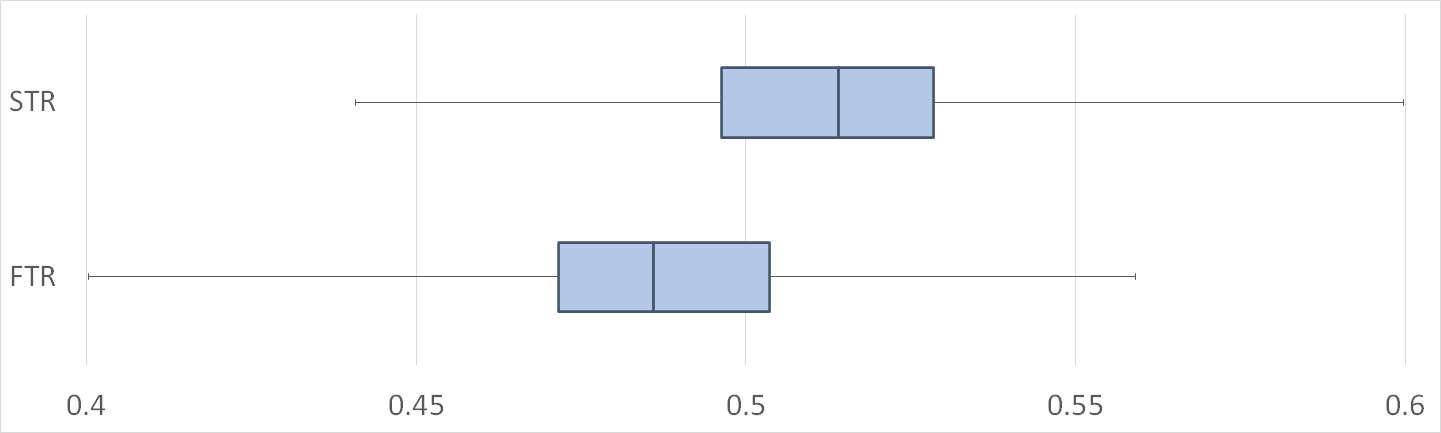
\includegraphics[width=\linewidth]{fig/Lang6_boxplot.png}
  \caption{箱ひげ図 : Lang6}
  \label{fig:Lang6_boxplot}
\end{figure}
\begin{table}[b]
  \centering
  \caption{Lang6バグのSTR, FTR}
  \label{tab:Lang6}
  \begin{tabular}{l|llllll} \hline\hline
    評価指標 & AVG         & MIN & 1Q & MED & 3Q & MAX   \\\hline
    STR & 0.5117 & 0.4409 & 0.4964 & 0.5140 & 0.5284 & 0.5997  \\
    FTR & 0.4883 & 0.4003 & 0.4716 & 0.4860 & 0.5036 & 0.5591 \\\hline\hline
  \end{tabular}
\end{table}
\begin{figure}[t]
  \centering
  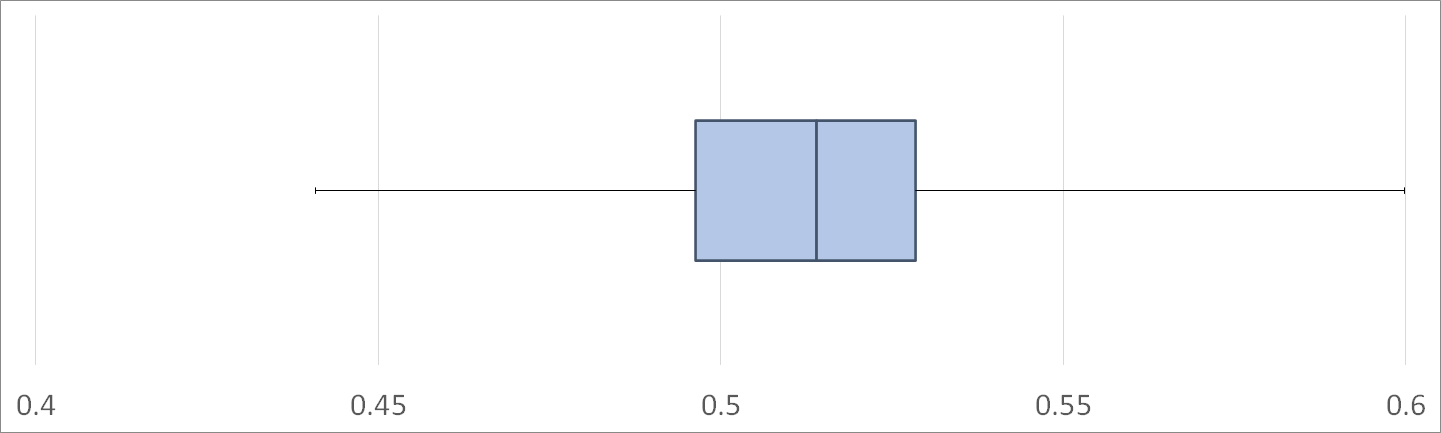
\includegraphics[width=\linewidth]{fig/Lang6_boxplot_STR.png}
  \caption{STRの箱ひげ図 : Lang6}
  \label{fig:Lang6_boxplot_STR}
\end{figure}
\begin{figure}[t]
  \centering
  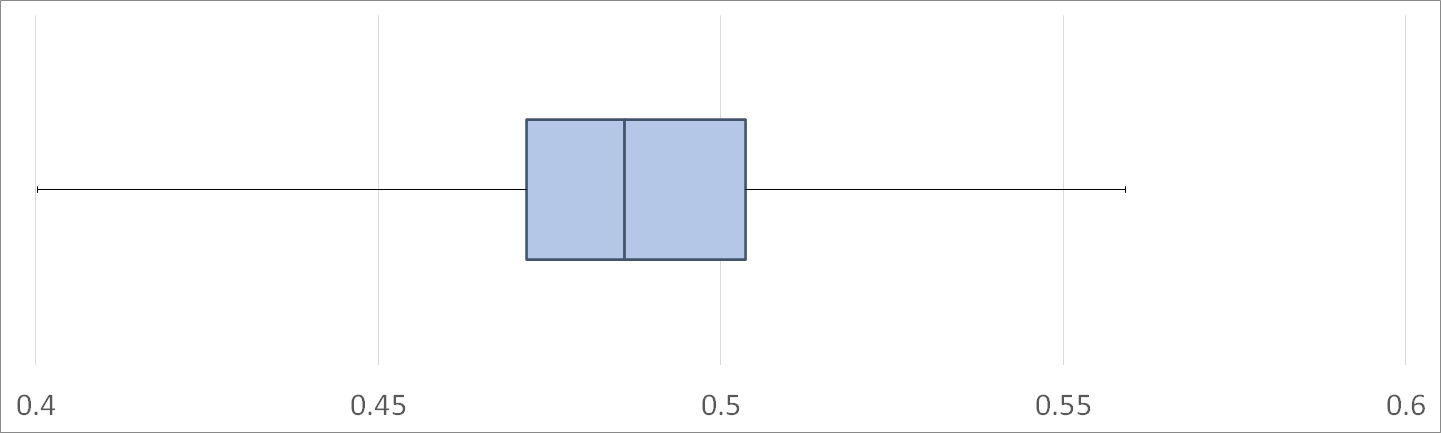
\includegraphics[width=\linewidth]{fig/Lang6_boxplot_FTR.png}
  \caption{FTRの箱ひげ図 : Lang6}
  \label{fig:Lang6_boxplot_FTR}
\end{figure}
\subsubsection{Lang22}
次いで,図\ref{fig:Lang22_boxplot}にLang22におけるSTRとFTRの箱ひげ図を示す.この結果からわかることとして,他のバグに比べてパッチの生成に多くの時間および操作を要した.そのため,他のバグに比べるとSTR,FTRのいずれの値も小さくなっている.とりわけFTRの値が0.03程度と非常に小さい値を得た.
\begin{figure}[t]
  \centering
  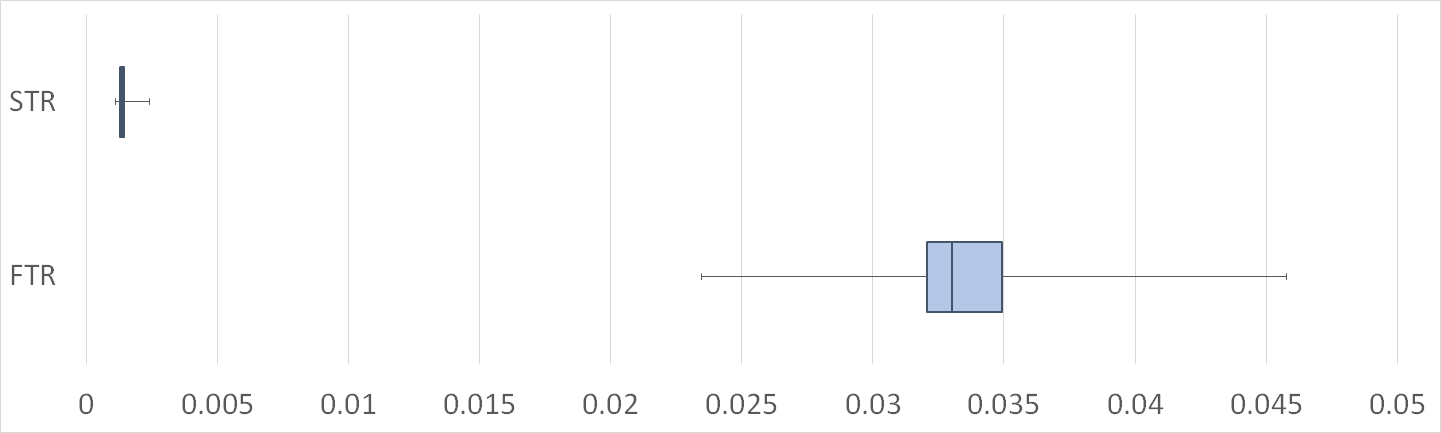
\includegraphics[width=\linewidth]{fig/Lang22_boxplot.png}
  \caption{箱ひげ図 : Lang22}
  \label{fig:Lang22_boxplot}
\end{figure}
\begin{table}[b]
  \centering
  \caption{Lang22バグのSTR, FTR}
  \label{tab:Lang22}
  \begin{tabular}{l|llllll} \hline\hline
    評価指標 & AVG         & MIN & 1Q & MED & 3Q & MAX   \\\hline
    STR & 0.001476 & 0.001096 & 0.001291 & 0.001354 & 0.001458 & 0.002418  \\
    FTR & 0.03432 & 0.02346 & 0.03208 & 0.03304 & 0.03492 & 0.04578 \\\hline\hline
  \end{tabular}
\end{table}
\begin{figure}[t]
  \centering
  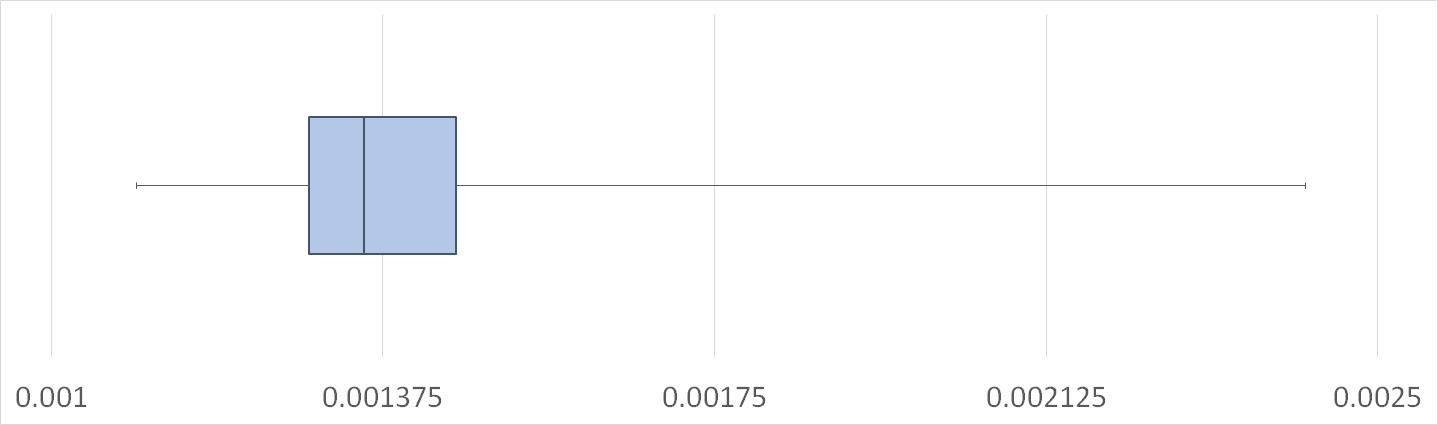
\includegraphics[width=\linewidth]{fig/Lang22_boxplot_STR.png}
  \caption{STRの箱ひげ図 : Lang22}
  \label{fig:Lang22_boxplot_STR}
\end{figure}
\begin{figure}[t]
  \centering
  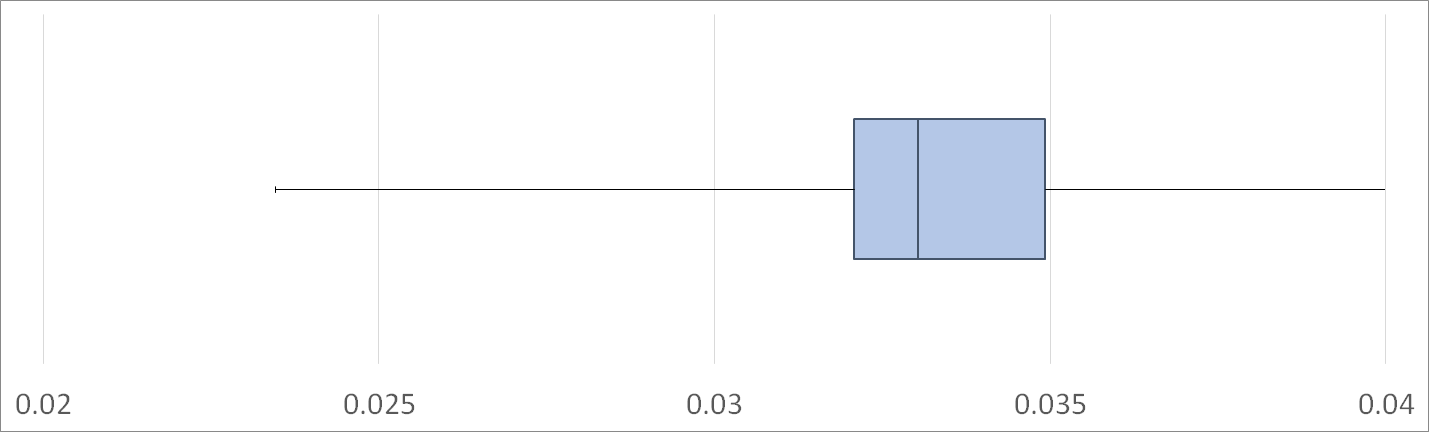
\includegraphics[width=\linewidth]{fig/Lang22_boxplot_FTR.png}
  \caption{FTRの箱ひげ図 : Lang22}
  \label{fig:Lang22_boxplot_FTR}
\end{figure}
\subsubsection{Lang25}
次に,図\ref{fig:Lang25_boxplot}にLang25におけるSTRとFTRの箱ひげ図を示す.このバグにおける特徴として,FTRの値が平均して0.8程度と高い数値を示している点があげられる.一方で,STRの値は0.1程度にとどまった.
\begin{figure}[t]
  \centering
  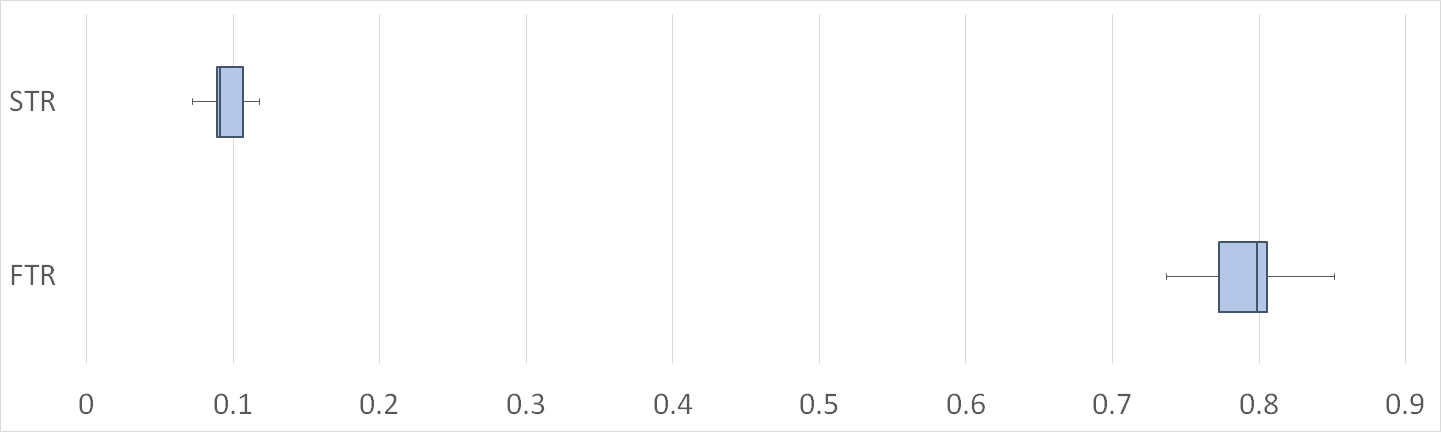
\includegraphics[width=\linewidth]{fig/Lang25_boxplot.png}
  \caption{箱ひげ図 : Lang25}
  \label{fig:Lang25_boxplot}
\end{figure}
\begin{table}[b]
  \centering
  \caption{Lang25バグのSTR, FTR}
  \label{tab:Lang25}
  \begin{tabular}{l|llllll} \hline\hline
    評価指標 & AVG         & MIN & 1Q & MED & 3Q & MAX   \\\hline
    STR & 0.09386 & 0.07261 & 0.08936 & 0.09106 & 0.1070 & 0.1177  \\
    FTR & 0.7986 & 0.7371 & 0.7725 & 0.7989 & 0.8053 & 0.8512 \\\hline\hline
  \end{tabular}
\end{table}
\begin{figure}[t]
  \centering
  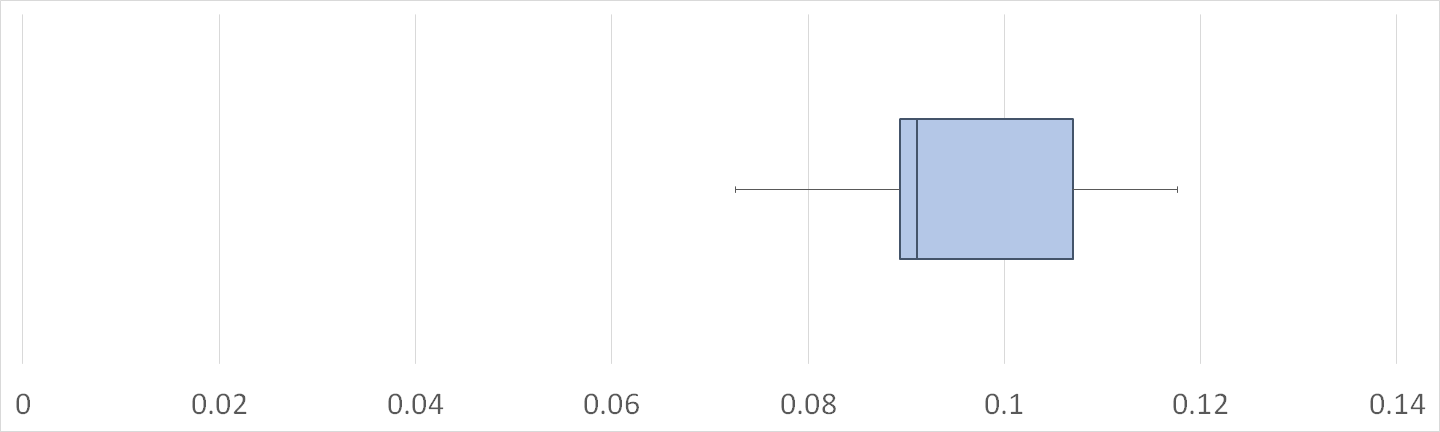
\includegraphics[width=\linewidth]{fig/Lang25_boxplot_STR.png}
  \caption{STRの箱ひげ図 : Lang25}
  \label{fig:Lang25_boxplot_STR}
\end{figure}
\begin{figure}[t]
  \centering
  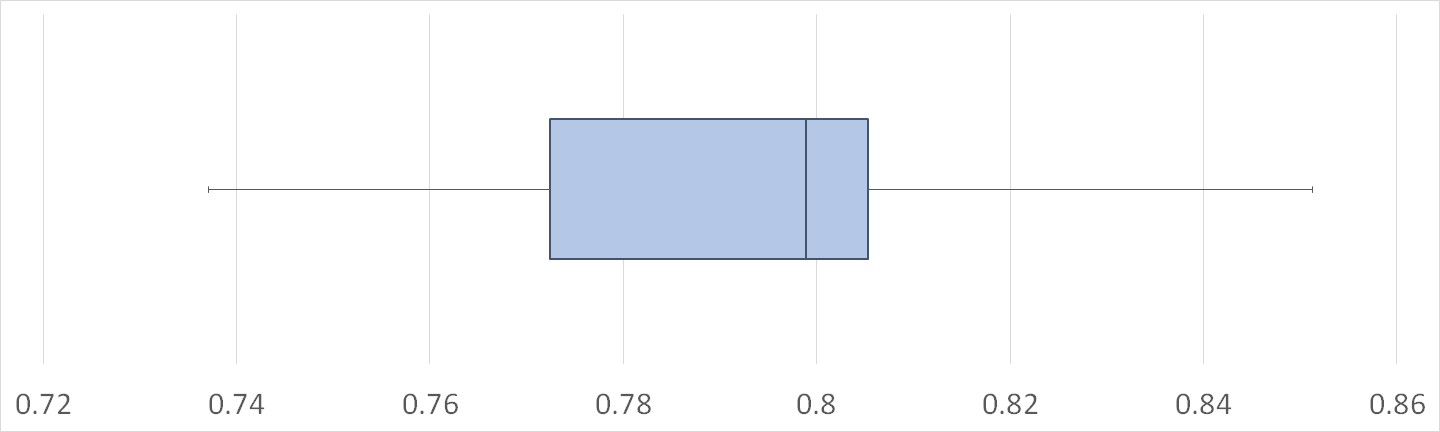
\includegraphics[width=\linewidth]{fig/Lang25_boxplot_FTR.png}
  \caption{FTRの箱ひげ図 : Lang25}
  \label{fig:Lang25_boxplot_FTR}
\end{figure}
\subsubsection{Lang39}
次に,図\ref{fig:Lang39_boxplot}にLang39におけるSTRとFTRの箱ひげ図を示す.このバグにおいても,Lang25ほどではないものの,FTRが0.6付近と高い値を得た.一方で,STRの値は0.02程度とFTRよりも著しく低い値となった.
\begin{figure}[t]
  \centering
  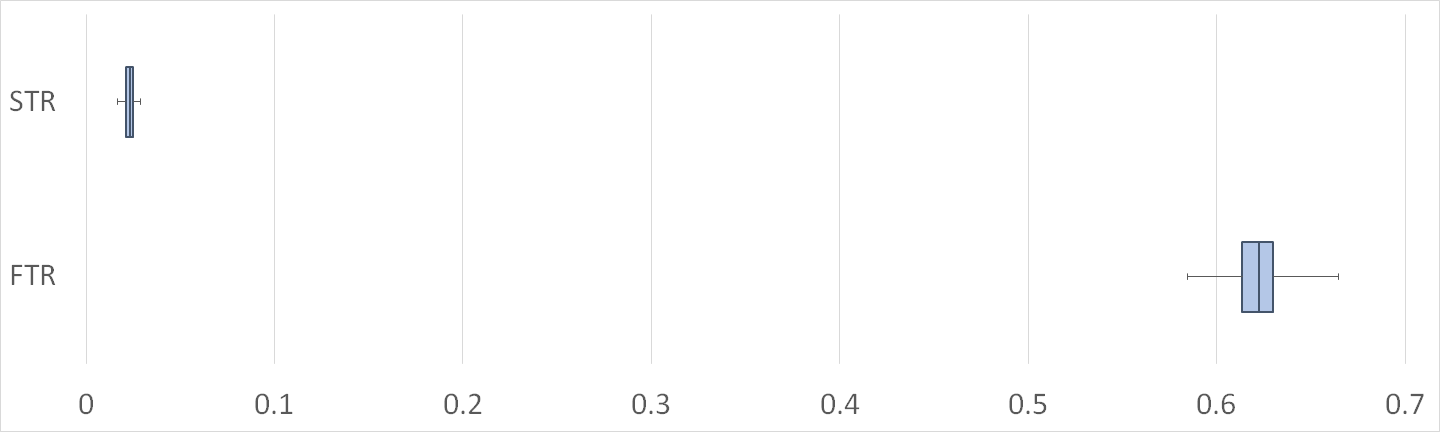
\includegraphics[width=\linewidth]{fig/Lang39_boxplot.png}
  \caption{箱ひげ図 : Lang39}
  \label{fig:Lang39_boxplot}
\end{figure}
\begin{table}[b]
  \centering
  \caption{Lang39バグのSTR, FTR}
  \label{tab:Lang39}
  \begin{tabular}{l|llllll} \hline\hline
    評価指標 & AVG         & MIN & 1Q & MED & 3Q & MAX   \\\hline
    STR & 0.02406 & 0.01645 & 0.02105 & 0.02326 & 0.02510 & 0.02873  \\
    FTR & 0.6218 & 0.5847 & 0.6137 & 0.6224 & 0.6299 & 0.6644 \\\hline\hline
  \end{tabular}
\end{table}
\begin{figure}[t]
  \centering
  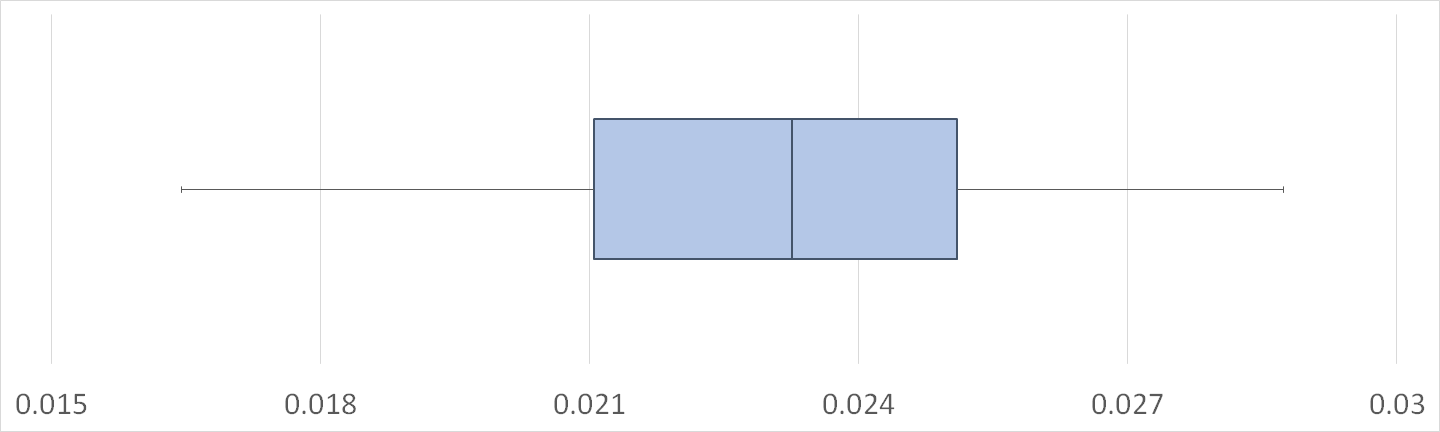
\includegraphics[width=\linewidth]{fig/Lang39_boxplot_STR.png}
  \caption{STRの箱ひげ図 : Lang39}
  \label{fig:Lang39_boxplot_STR}
\end{figure}
\begin{figure}[t]
  \centering
  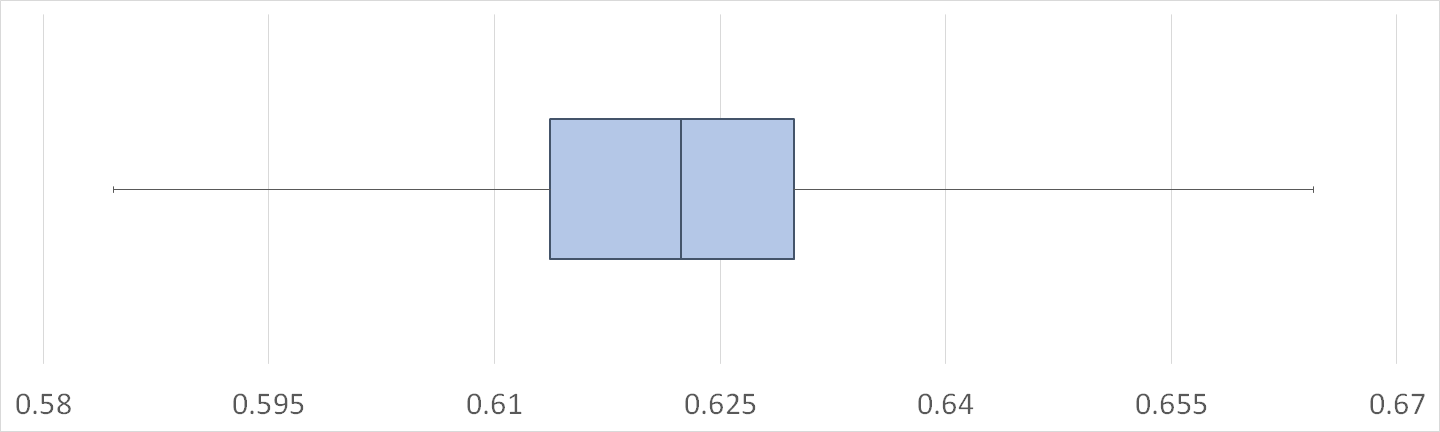
\includegraphics[width=\linewidth]{fig/Lang39_boxplot_FTR.png}
  \caption{FTRの箱ひげ図 : Lang39}
  \label{fig:Lang39_boxplot_FTR}
\end{figure}
\subsubsection{実験結果の総括}
最後に,今回実験の対象とした4つのバグについて,得られた結果を比較しながら論述する.
まず,STR(図\ref{fig:summary_STR})について,先述したとおりLang6においては0.5を超える値を記録している.一方で,その他のバグにおいてはいずれにおいても平均値が0.1を下回った.このことは,解に関係する個体の全体に占める生成時間が1割未満であることを意味する.
次に,FTR(図\ref{fig:summary_FTR})について,0.03程度の値を得たLang22を除くと,5割~8割程度の値に落ち着いた.特にLang25においてはビルドに失敗した個体の全体に占める生成時間が8割を超えることもあることが分かった.
\begin{figure}[t]
  \centering
  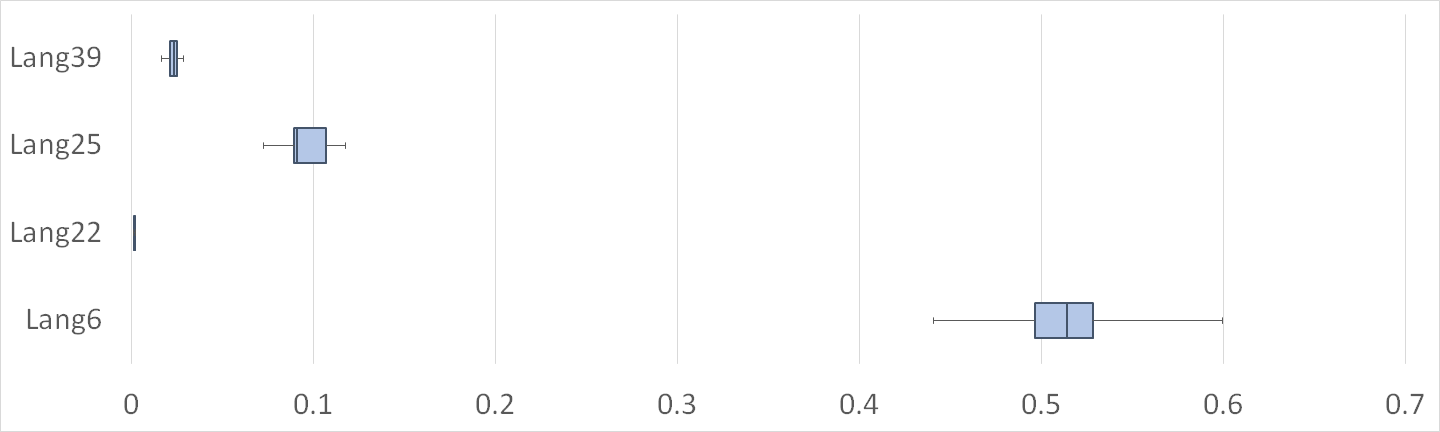
\includegraphics[width=\linewidth]{fig/summary_STR.png}
  \caption{4つのバグにおけるSTRの箱ひげ図}
  \label{fig:summary_STR}
\end{figure}
\begin{figure}[t]
  \centering
  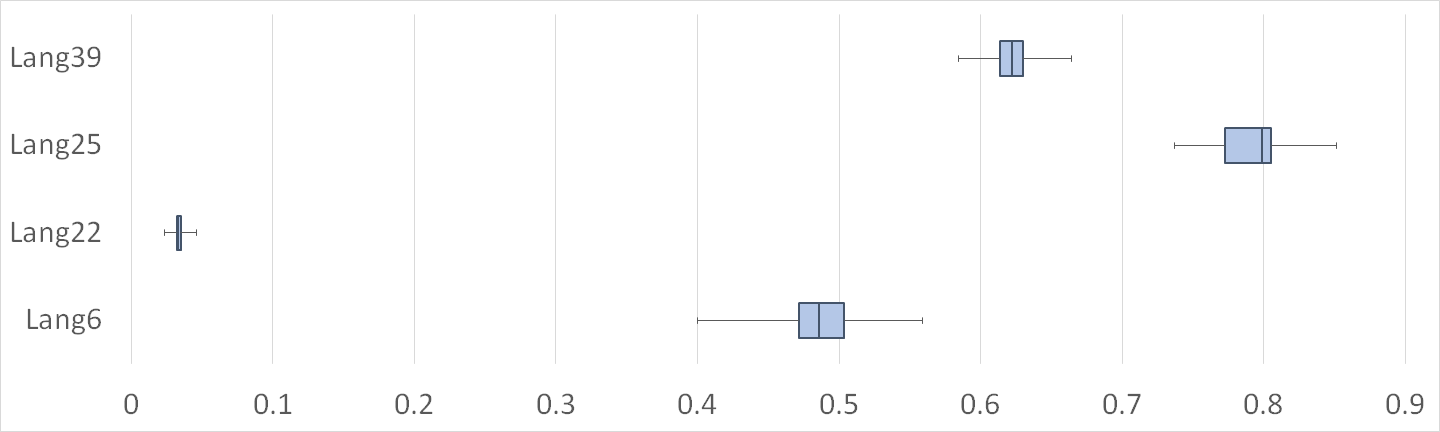
\includegraphics[width=\linewidth]{fig/summary_FTR.png}
  \caption{4つのバグにおけるFTRの箱ひげ図}
  \label{fig:summary_FTR}
\end{figure}
%%%%%%%%%%%%%%%%%%%%%%%%%%%%%%%%%%%%%%%%%%%%%%%%%%%%%%%%%%%%%%%%%%%%%%%%%%%%%%%%%%%%%%%%%%%%%%%%%%%
\clearpage
\section{考察}\label{sec:cons}
\ref{sec:exp}章では,1世代あたりの変異・交叉個体数を表\ref{tab:apr_setting}のように設定したが,この値を変更することでSTRおよびFTRの値に変化が見られるかを考察したい.
この章では,Lang39バグに対して,1世代あたりの個体数を変更した場合のSTRとFTRの値の影響を調査し,その結果に対する考察を述べる.
\subsection{比較対象の設定}
表\ref{tab:comparison}に\ref{sec:exp}章で行ったと比較対象となる実験の設定および生成時間に関係しない結果について相違点のある項目のみを示す.
\begin{table}[b]
  \centering
  \caption{比較実験の設定・結果}
  \label{tab:comparison}
  \begin{tabular}{l|ll} \hline\hline
    項目 & 比較元         & 比較対象                           \\\hline
    1世代ごとの変異個体数 & 70 & 5 \\
    1世代ごとの交叉個体数 & 30 & 2 \\
    サンプル数 & 40 & 30 \\
    生成個体数 & 300 & 541 \\
    ビルド失敗個体数 & 274 & 461 \\\hline\hline
  \end{tabular}
\end{table}
図\ref{fig:cons-STR}および図\ref{fig:cons-FTR},表\ref{tab:res-comparison-STR}および表\ref{tab:res-comparison-FTR}はそれぞれ比較実験におけるSTR・FTRの値を表した箱ひげ図および有効数字4桁の値である.ここで,Lang39Cは比較実験における素のデータを表すが,比較対象となった30回いずれの修正においても特定の1個体に費やした生成時間が他の生成時間に比べはるかに大きな値を記録した(いわゆる外れ値)ため,その個体の生成時間を除外したデータがLang39C2である.\\
なお,この個体は,ビルドには成功したが,解の個体の経路には含まれなかった.そのため,まずSTRについては,Lang39CとLang39が0.02前後の値をとったのに対し,Lang39C2は0.05とほか2つより高い値を記録した.一方でFTRについてはLang39Cがほかの2つに比べ半分未満の値をとった.\\
考察として,個体の生成時間に制限を設けた場合,制限時間を過ぎた個体の生成が中止された場合,その個体が解となる個体の親たりえない場合はSTRの値が向上するのではないかということがあげられる.
\begin{figure}[t]
  \centering
  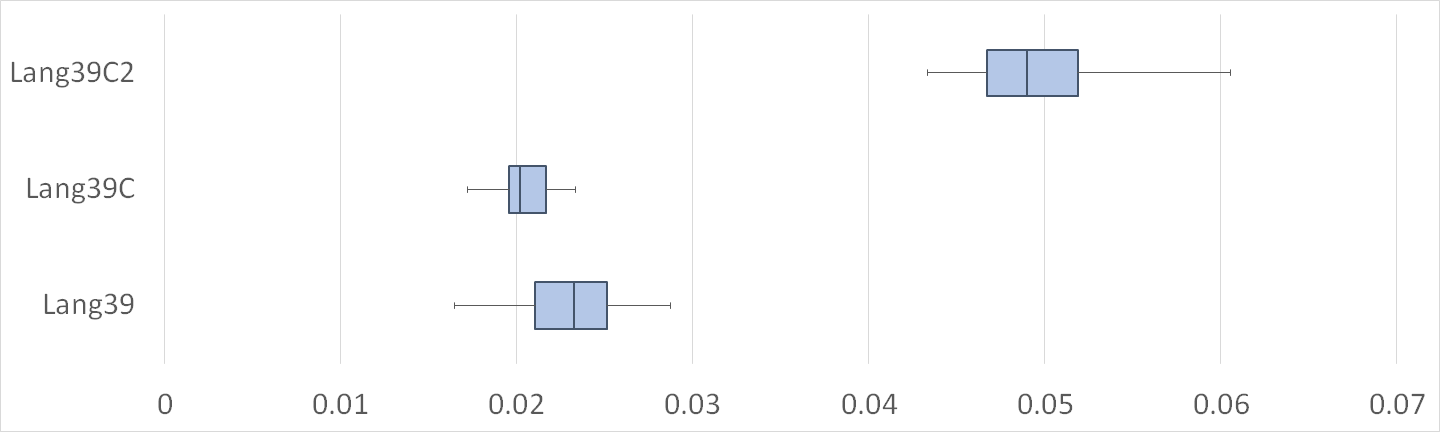
\includegraphics[width=\linewidth]{fig/cons_STR.png}
  \caption{Lang39バグにおける比較実験のSTR箱ひげ図}
  \label{fig:cons-STR}
\end{figure}
\begin{figure}[t]
  \centering
  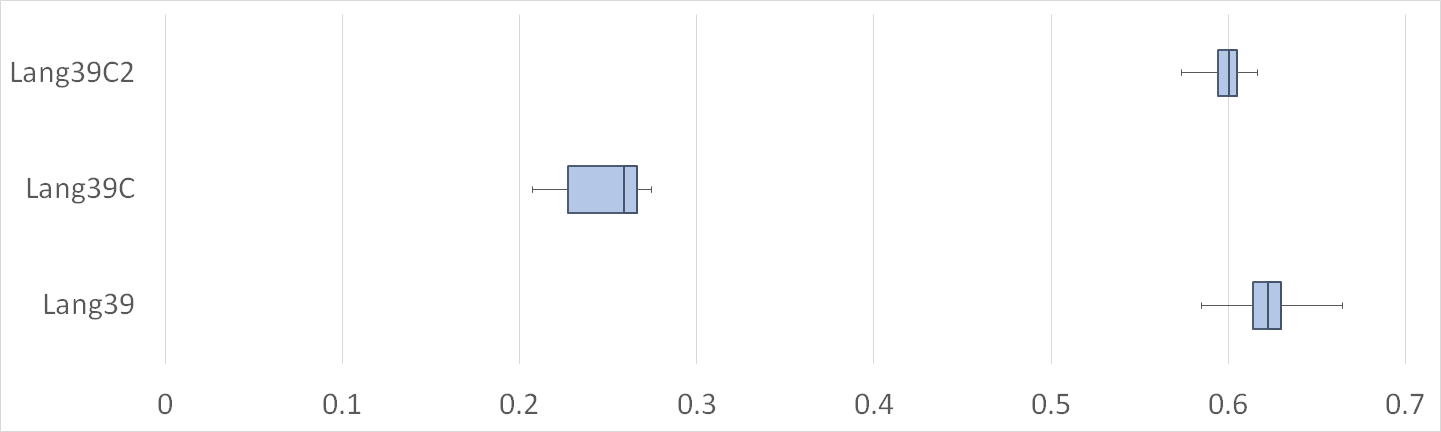
\includegraphics[width=\linewidth]{fig/cons_FTR.png}
  \caption{Lang39バグにおける比較実験のFTR箱ひげ図}
  \label{fig:cons-FTR}
\end{figure}
\begin{table}[b]
  \centering
  \caption{Lang39バグにおける比較実験のSTR}
  \label{tab:res-comparison-STR}
  \begin{tabular}{l|llllll} \hline\hline
    評価指標 & AVG         & MIN & 1Q & MED & 3Q & MAX   \\\hline
    Lang39C2 & 0.04953 & 0.04334 & 0.04671 & 0.04898 & 0.05187 & 0.06052 \\
    Lang39C & 0.02045 & 0.01719 & 0.01958 & 0.02017 & 0.02167 & 0.02334 \\
    Lang39 & 0.02406 & 0.01645 & 0.02105 & 0.02326 & 0.02510 & 0.02873  \\\hline\hline
  \end{tabular}
\end{table}
\begin{table}[b]
  \centering
  \caption{Lang39バグにおける比較実験のFTR}
  \label{tab:res-comparison-FTR}
  \begin{tabular}{l|llllll} \hline\hline
    評価指標 & AVG         & MIN & 1Q & MED & 3Q & MAX   \\\hline
    Lang39C2 & 0.5987 & 0.5735 & 0.5940 & 0.6006 & 0.6049 & 0.6163 \\
    Lang39C & 0.2480 & 0.2070 & 0.2272 & 0.2587 & 0.2662 & 0.2746   \\
    Lang39 & 0.6218 & 0.5847 & 0.6137 & 0.6224 & 0.6299 & 0.6644 \\\hline\hline
  \end{tabular}
\end{table}
%次に,\ref{sec:exp}章で行った実験の結果から,各バグおよび全体的傾向について考察する.
%まず,ビルドに失敗した個体の割合について考察を行うために各バグにおけるFVRを次の式で定義する.
%\begin{equation}
%\label{eq:FVR} {\rm FVR} =  \frac{ビルドに失敗した個体の総数}{対象プログラムの個体の総数}
%\end{equation}
%表\ref{tab:FVR}に,各バグにおけるFVRの値,FTRとFVRの積およびFTRをFVRで割った値を示す.
%\begin{table}[b]
%  \centering
%  \caption{考察 : 各バグにおけるFVR}
%  \label{tab:FVR}
%  \begin{tabular}{l|llll} \hline\hline
%   バ名 & Lang6  & Lang22 & Lang25 & Lang39   \\\hline
%    FVR & 0.8750 & 0.8189 & 0.9474 & 0.9133  \\
%    FTR & 0.4883 & 0.03432 & 0.7986 & 0.6218 \\
%    FTR $\times$ FVR & 0.4272 & 0.02811 & 0.7566 & 0.5679 \\
%    FTR / FVR & 0.5580 & 0.04191 & 0.8430 & 0.6808 \\\hline\hline
%  \end{tabular}
%\end{table}
%この表から読み取れることとして,FTRをFVRで割った値は1に近い値をとるのではないかと予想したが,実際はFTRに比べてわずかに値が上がる程度であり予想ほど近づくことはなかった.
%%%%%%%%%%%%%%%%%%%%%%%%%%%%%%%%%%%%%%%%%%%%%%%%%%%%%%%%%%%%%%%%%%%%%%%%%%%%%%%%%%%%%%%%%%%%%%%%%%%
\clearpage
\section{妥当性の脅威}\label{sec:threat}
\ref{sec:exp}章における実験において考えうる妥当性の脅威について論ずる.この実験では内的要因と外的要因に大別される.
まず内的要因として,今回実行した環境とは異なる環境において実行した際に算出されるSTRとFTRの値が異なる可能性がある点があげられる.また,実行時に他のタスクによりメモリが占領されている場合,普段と異なる値が算出されうる点があげられる.\\
次に外的要因として,今回対象としたバグを含むプログラムは生成個体数が多いもので600程度と比較的少なかったが,大規模なプログラムにおいて何万といった個体が生成されたときにSTRとFTRの値が大きく異なる可能性がある点があげられる.
% また,kGenProg以外のツールを用いて実験を行った場合,
%%%%%%%%%%%%%%%%%%%%%%%%%%%%%%%%%%%%%%%%%%%%%%%%%%%%%%%%%%%%%%%%%%%%%%%%%%%%%%%%%%%%%%%%%%%%%%%%%%%
\clearpage
\section{今後の課題}\label{sec:ftrclg}
本研究においては,探索ベースで遺伝的アルゴリズムを採用した\kgp を対象に個体の生成時間計測を行ったが,
\subsection{APRツールによる生成時間の違いの検証}
本研究で用いたAPRツールは探索ベースで遺伝的アルゴリズムを採用した\kgp を対象に個体の生成時間計測を行ったが,遺伝的アルゴリズムでないほかの探索ベースのAPRツールや意味論ベースのAPRツールにおいて時間計測を行う.
\subsection{時間計測を行う対象プロジェクトの拡張}
本研究では,Defects4JのLangバグのうち,4つのバグを対象としてSTRとFTRの計算を行った.今後は,Defects4Jのほかのバグやその他の対象について時間研究を行う.
%%%%%%%%%%%%%%%%%%%%%%%%%%%%%%%%%%%%%%%%%%%%%%%%%%%%%%%%%%%%%%%%%%%%%%%%%%%%%%%%%%%%%%%%%%%%%%%%%%%
\clearpage
\section{おわりに}\label{sec:concl}
本稿では,APRツールに対して個体の生成時間を計測する機能を追加し,実際のバグに対してSTRとFTRという2つの指標を定義した.
さらに実際のバグに対して指標を計算する実験を行うことで時間的コストの評価を行った.
結果として,多くのバグにおいて解の個体生成にかかる時間は,ビルドに失敗した個体の生成にかかる時間に比べて	はるかに小さいことが示された.しかし,Lang6バグのように,例外的な値をとるプログラムも存在する.そこで,将来的な研究ではビルドに失敗した個体に対する解の個体の時間的生成効率の改善を行う,より多くのバグに対する提案指標の検証を行う.
% =================================================================================================
% 謝辞
\clearpage
\acknowledgement

本研究を進めるにあたり,多くの方々からご支援およびご助言を賜りました.

楠本 真二 教授には,本研究を快く快諾し,暖かく見守ってくださりました.
心より感謝申し上げます.

肥後 芳樹 教授には,議論を重ねに重ね,本研究の完成のご支援及び的確なご助言を賜りました.
心より感謝申し上げます.

柗本 真佑 助教には,テーマが決まらず途方に暮れていた際,鋭くも的確なご助言を賜りました.
深く感謝いたします.

古藤 寛大先輩には,困難に直面した際いつも迅速にご助言を賜り感謝してもしきれません.

本研究に至るまでに,講義,演習等でお世話になりました大阪大学基礎工学部情報科学科の諸先生方に,御礼申し上げます.

最後に,これまでお世話になりました家族,小中高校の教員方,その他すべての方に感謝申し上げます.
% =================================================================================================
% 参考文献
\clearpage
\bibliographystyle{junsrt}
\bibliography{references.bib}

\end{document}
